% Autor: Leonhard Segger, Alexander Neuwirth
% Datum: 2017-10-30
\documentclass[
	% Papierformat
	a4paper,
	% Schriftgröße (beliebige Größen mit „fontsize=Xpt“)
	12pt,
	% Schreibt die Papiergröße korrekt ins Ausgabedokument
	pagesize,
	% Sprache für z.B. Babel
	ngerman
]{scrartcl}

% Achtung: Die Reihenfolge der Pakete kann (leider) wichtig sein!
% Insbesondere sollten (so wie hier) babel, fontenc und inputenc (in dieser
% Reihenfolge) als Erstes und hyperref und cleveref (Reihenfolge auch hier
% beachten) als Letztes geladen werden!

\usepackage{tikz}
\usetikzlibrary{calc,patterns,angles,quotes} % loads some tikz extensions\usepackage{tikz}
\usetikzlibrary{babel}

% Silbentrennung etc.; Sprache wird durch Option bei \documentclass festgelegt
\usepackage{babel}
% Verwendung der Zeichentabelle T1 (Sonderzeichen etc.)
\usepackage[T1]{fontenc}
% Legt die Zeichenkodierung der Eingabedatei fest, z.B. UTF-8
\usepackage[utf8]{inputenc}
% Schriftart
\usepackage{lmodern}
% Zusätzliche Sonderzeichen
\usepackage{textcomp}

% Mathepaket (intlimits: Grenzen über/unter Integralzeichen)
\usepackage[intlimits]{amsmath}
% Ermöglicht die Nutzung von \SI{Zahl}{Einheit} u.a.
\usepackage{siunitx}
% Zum flexiblen Einbinden von Grafiken (\includegraphics)
\usepackage{graphicx}
% Abbildungen im Fließtext
\usepackage{wrapfig}
% Abbildungen nebeneinander (subfigure, subtable)
\usepackage{subcaption}
% Funktionen für Anführungszeichen
\usepackage{csquotes}
\MakeOuterQuote{"}
% Zitieren, Bibliografie
\usepackage[sorting=none]{biblatex}


% Zur Darstellung von Webadressen
\usepackage{url}
%chemische Formeln
\usepackage[version=4]{mhchem}
% siunitx: Deutsche Ausgabe, Messfehler getrennt mit ± ausgeben
\usepackage{floatrow}
\floatsetup[table]{capposition=top}
\usepackage{float}
% Verlinkt Textstellen im PDF-Dokument
\usepackage[unicode]{hyperref}
% "Schlaue" Referenzen (nach hyperref laden!)
\usepackage{cleveref}
\sisetup{
	locale=DE,
	separate-uncertainty
}
\bibliography{BA-C-04_MP5_10-12-2018_References}

\begin{document}

	\begin{titlepage}
		\centering
		{\scshape\LARGE Versuchsbericht zu \par}
		\vspace{1cm}
		{\scshape\huge MP5 - Weiche Materie: Physik der
flüssigen Kristallen \par}
		\vspace{2.5cm}
		{\LARGE Gruppe BA-C-04 \par}
		\vspace{0.5cm}

		{\large Alexander Neuwirth (E-Mail: a\_neuw01@wwu.de) \par}
		{\large Leonhard Segger (E-Mail: l\_segg03@uni-muenster.de) \par}
		\vfill

		durchgeführt am 10.12.2018\par
		betreut von\par
		{\large Aaron Rigoni}

		\vfill

		{\large \today\par}
	\end{titlepage}
	\tableofcontents
	\newpage


	\section{Kurzfassung}
	% Hypothese	und deren Ergebnis, wenn Hypothese ist, dass nur Theorie erfüllt, sagen: Erwartung: Theorie aus einführung (mit reflink) erfüllt
	% Ergebnisse, auch Zahlen, mindestens wenn's halbwegs Sinn ergibt
	% Was wurde gemacht
	% manche leute wollen Passiv oder "man", manche nicht

	\section{Theorie}
	%TODO v
	% wdh. Texte
	% wdh. Besprechung
	% FRagen aus Einleitung
	\section{Methoden}
	% Bilder von der Website klauen
	% einer will Präsens
	%TODO I guess hier der LCD-Bau, weil sonst (bis auf Diskussion) macht es net so viel Sinn

	\section{Ergebnisse und Diskussion}
	\subsection{Bestimmung der Kennlinien der LC-Displays}
	\subsubsection{Unsicherheiten}
	Beide Spannungen werden von einer digitalen Anzeige abgelesen.
	Mit einer Rechteckverteilung ergibt sich für die Spannung $U_{LCD}$ mit welcher das Display betrieben wird $u(U_{LCD})=\SI{0.00003}{V}$ und für die der Photodiode $u(U_{Ph})=\SI{0.0003}{V}$.
	Da beide Anzeigen stark in den letzten Ziffern schwanken, wird die Breite der Schwankungen mit
	\begin{itemize}
		\item $u(U_{LCD})=\SI{0.001}{V}$
		\item $u(U_{Ph})=\SI{0.003}{V}$
	\end{itemize}
	abgeschätzt, wohingegen die Displayunsicherheiten verschwinden.
	Da die Schwankungen der Diodenspannung deutlich größer im Bereich von 10\% bis 90\% Transmission ist, wird hierfür die doppelte Unsicherheit verwendet.
	\subsubsection{Beobachtung und Datenanalyse}
	%TODO Allg Beob
	Beim Betrieb des selbstgebauten und industriellen Displays lässt sich feststellen, dass sie dunkler, bzw. weniger lichtdurchlässig, werden, wenn man die Spannung erhöht.
	Das selbstgebaute Display flimmert und ist nicht so dunkel wie das Industrie-Display.

	Um von der an der Photodiode gemessenen Spannung auf auf die relative Transmission zu schließen wird %TODO erklären wie Diode Licht intensität messen tut? %TODO von der an der...
	\begin{equation}
			T = \frac{U-U_{max}}{U_{max}-U_{min}}
	\end{equation}
	verwendet. Wobei sich die kombinierte Standardunsicherheit
	\begin{align*}
		u(T) &= \sqrt{\sum_{i}\left(\frac{\partial T}{\partial x_i} u(x_i)\right)^2}\\
		&= \sqrt{\left(\frac{u(U)}{U_{max}-U_{min}}\right)^2+\left(\frac{u(U_{max})(U_{min}-U)}{(U_{max}-U_{min})^2}\right)^2+\left(\frac{u(U_{min})(U-U_{max})}{(U_{max}-U_{min})^2}\right)^2} \\
		&=	\frac{\sqrt{ (\alpha^2+1) (U_{max}-U_{min})^2+2U_{max}U_{min}+2U(U-U_{max}-U_{min})}}{(U_{max}-U_{min})^2} u(U_{max}) \\
	\end{align*}
	mit
	\begin{equation*}
			u(U)=\alpha u(U_{max})=\alpha u(U_{min})
	\end{equation*}
	ergibt.
	Mittels der Werte aus \cref{tb_maxmin} lassen sich die Messpunkte in die Kennlinien in \cref{fig_industry} und \cref{fig_selfmade} transformieren.
\begin{table}[H]
		\centering
		\begin{tabular}{ c | c | c }
			 & industriell & selbstgebaut \\ \hline
			$U_{max}$ & \SI{2.414+-0.003}{V} & \SI{1.866+-0.003}{V} \\
			$U_{min}$ & \SI{0.047+-0.003}{V} & \SI{0.360+-0.003}{V} \\
	\hline
		\end{tabular}
		\caption{Maximal und minimal gemessene Spannungen beim Bestimmen der Kennlinie des selbstgebauten und industriell gefertigten Displays mittels einer Photodiode.}
		\label{tb_maxmin}
\end{table}

	\begin{figure}[H]
			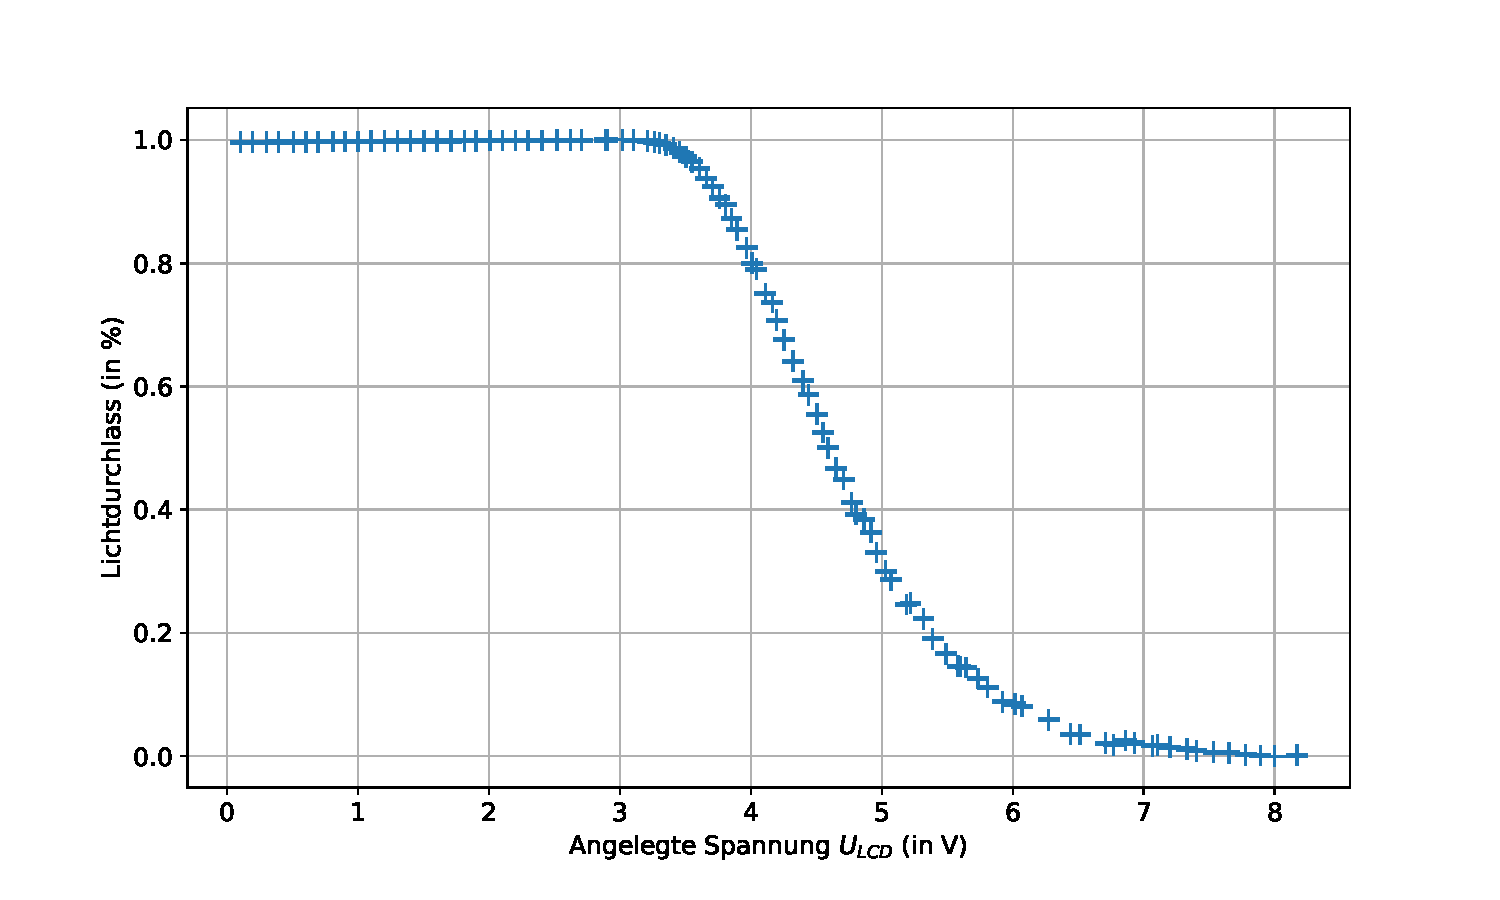
\includegraphics[width=1\linewidth]{images/industry.pdf}
			\caption{Kennlinie des industriell hergestellten LC-Displays.
			Die schwarze Senkrechte beschreibt die Schwellspannung, welche mindestens am Display anliegen muss um eine Veränderung messen zu können.
			Die rote(grüne) bespreibt dagegen eine Transmission von 90\%(10\%) durch das Diplay.  %TODO meh deutsch
			}
			\label{fig_industry}
	\end{figure}
	\begin{figure}[H]
			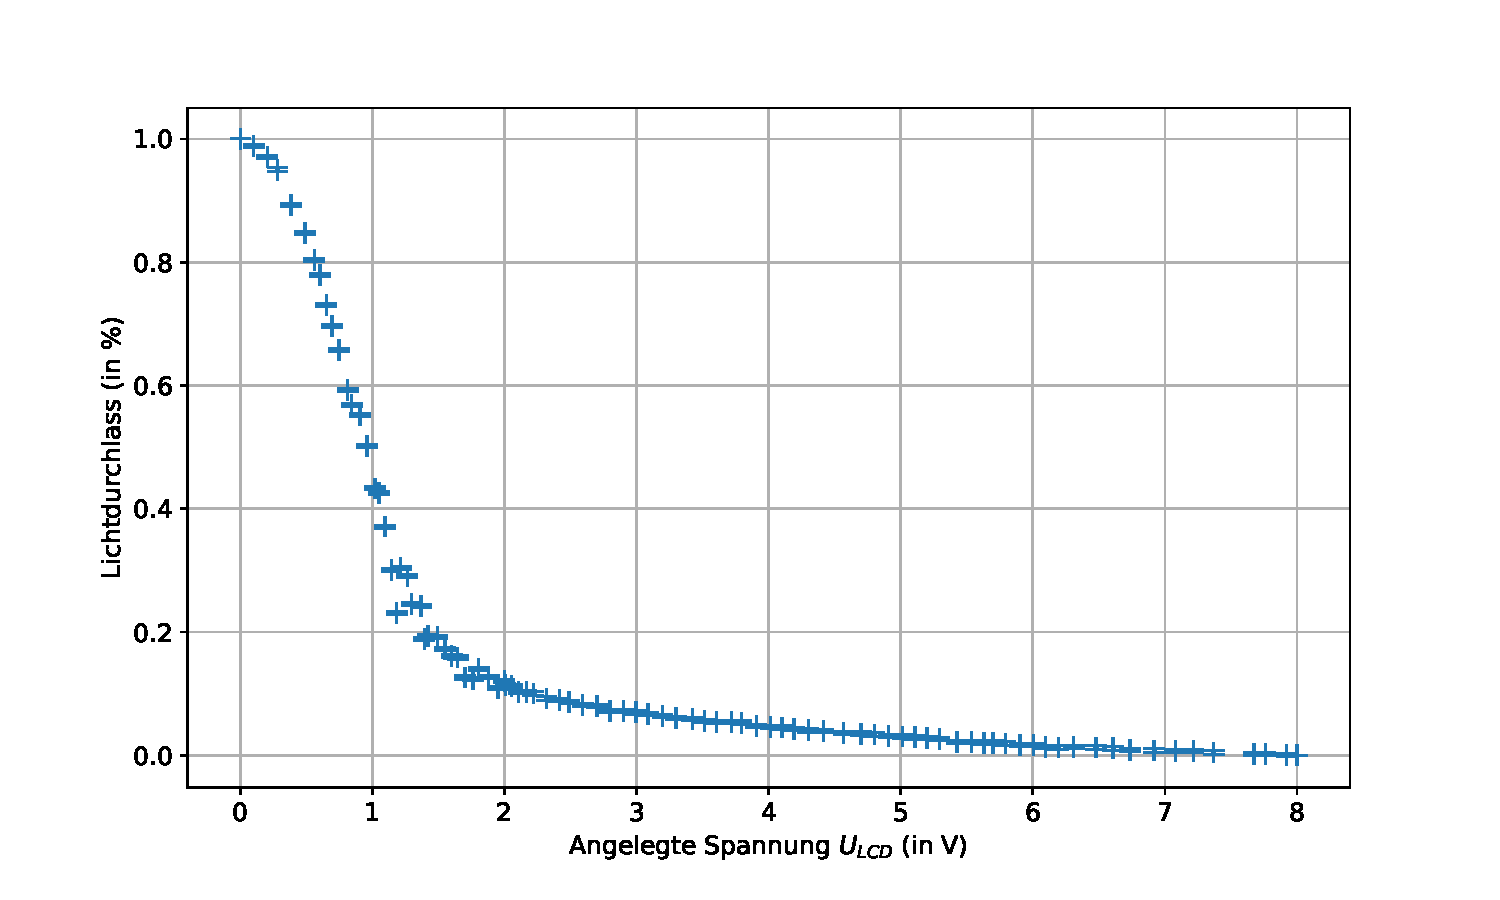
\includegraphics[width=1\linewidth]{images/selfmade.pdf}
			\caption{Kennlinie des selbstgebauten LC-Displays.
			Die schwarze Senkrechte beschreibt die Schwellspannung, welche mindestens am Display anliegen muss um eine Veränderung messen zu können.
			Die rote(grüne) bespreibt dagegen eine Transmission von 90\%(10\%) durch das Diplay.  %TODO meh deutsch
			}
			\label{fig_selfmade}
	\end{figure}
	Aus den Kennlinien lassen sich die Kenngrößen aus \cref{tb_kenngroessen} bestimmen.
	\begin{table}[H]
		\centering
		\begin{tabular}{ c | c | c }
			 & industriell & selbstgebaut \\ \hline
			$\Delta U=U_{10}-U_{90}$&\SI{2.0009+-0.0016}{V}&\SI{1.8348+-0.0016}{V} \\
			$U_{th}$ & \SI{3.211+-0.0012}{V} & \SI{0.0016+-0.0012}{V} \\
			\hline
		\end{tabular}
		\caption{Kenngrößen des selbstgebauten und industriell gefertigten Displays.}
		\label{tb_kenngroessen}
\end{table}

	\subsubsection{Diskussion}
	%TODO Schwellspannung Unterschied U_th Grund?Nutzen?
	%TODO U_th hängt von Anisotropie Delta epsilon ab (vgl. -> Einleitung)
	%TODO Delta U ist bei selfmade kleiner => gut für Kontrastreiche Hell-Dunkel Displays, aber! selfmade beim ist die absolute Diodenspannung immernoch 10x heller. (soll des iwo in  Beobachtung?, passt jedenfalls zu Augen-beobachtung)
	%TODO U_max U_min diskussion
	\subsection{Bestimmung der kritischen Temperatur eines Flüssigkristalls} %TODO kritische Temperatur vs Klärpunkt
	\subsubsection{Unsicherheiten}
	Die Temperatur des Flüssigkristalls wird mit einem Thermometer mit einer Nachkommastelle gemessen, wodurch sich eine Unsicherheit von $u(T)=\SI{0.03}{\degree C}$.
	Die Unsicherheit des Abstands der aufgespalteten Strahlen des Lasers wird mit $u(d)=\SI{1.7}{mm}$ abgeschätzt.
	Diese setzt sich aus der Größe des Laserstrahls auf dem Millimeterpapier und der instabilen Halterung des Laserpointers zusammen.
	\subsubsection{Beobachtung und Datenanalyse}
	Beim Steigern der Temperatur des Flüssigkristalls zeigt sich zunächst kaum eine Änderung in der Aufspaltung des Laserstrahls.
	Erst beim Überschreiten einer Grenztemperatur ändert sich die milchige Farbe des Kristalls zu einer klaren Flüssigkeit.
	Zeitgleich verschwinden die zwei Strahlen und es findet sich nur noch ein Strahl zwischen den ursprünglichen Strahlen.

	Der gemessene Abstand der Laserstrahlen ist in \cref{fig_laser} abhängig von der Temperatur dargestellt.
	Die kritische Temperatur $T_C$ liegt ca. bei \SI{36+-0.6}{\degree C}.
		\begin{figure}[H]
			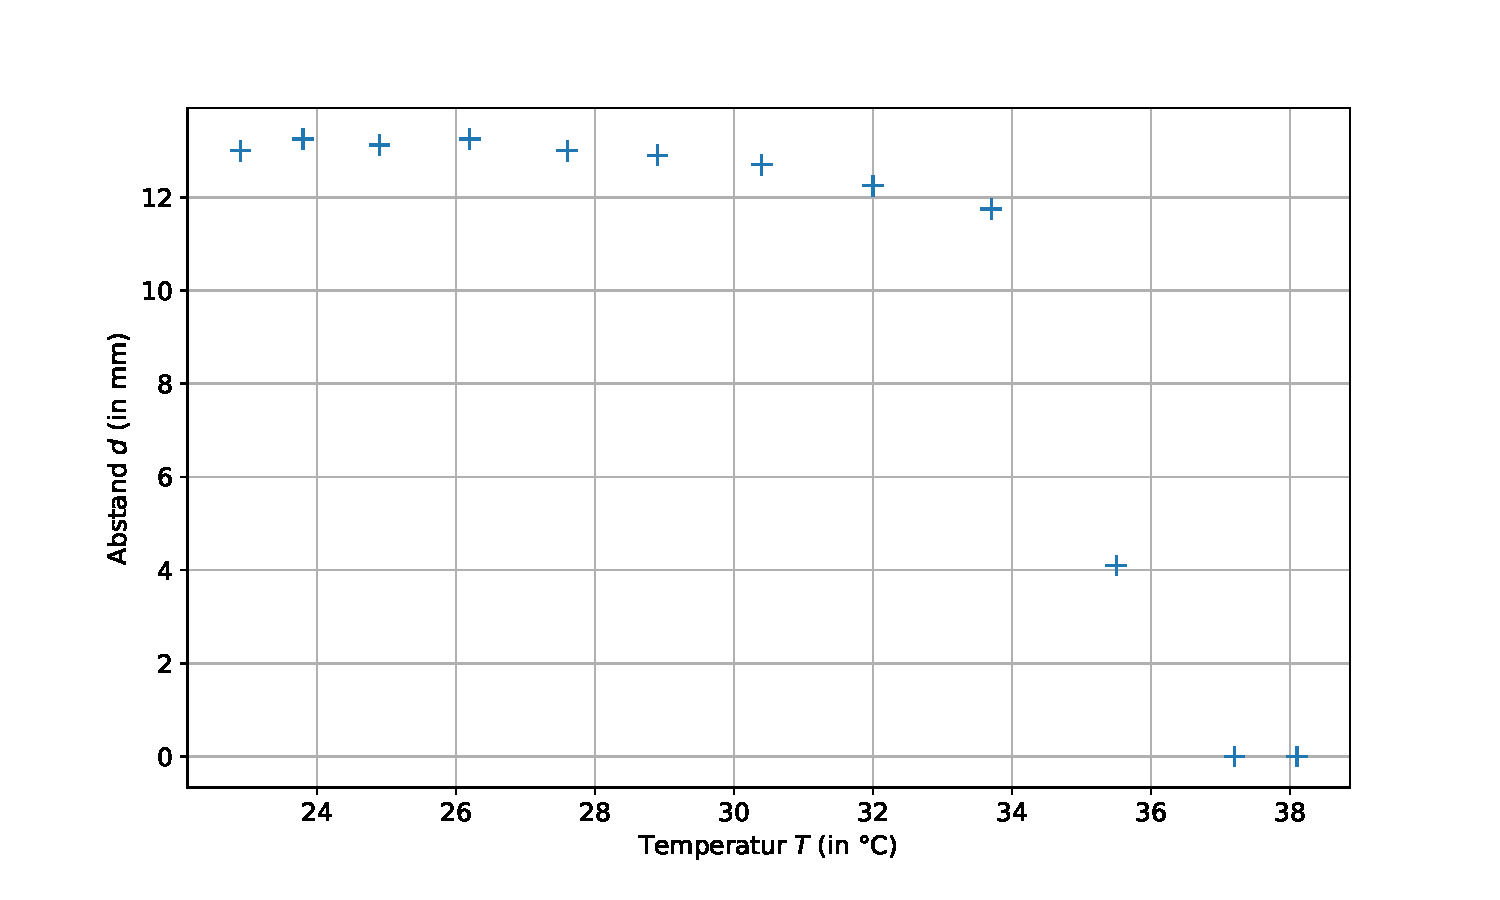
\includegraphics[width=1\linewidth]{images/laser.pdf}
			\caption{
			Temperaturabhängigkeit des Flüssigkristalls.
			Die Verbindungslinien zwischen den Messpunkten dienen lediglich der Veranschaulichung des Verlaufs.
			}
			\label{fig_laser}
	\end{figure}
	\subsubsection{Diskussion}
	%TODO ggf. erwähnen das Fehler zu groß abgeschätz  wurde, denke eig. aber des macht net so Sinn.
	%TODO Verlauf ist so wie erwartet. (inklusiver der kleinen Annäherung vor dem Anitsplit)
	%TODO Methode nicht geeignet um Kristische Temperatur exakt zu bestimmen, besser wenniger Flüssigkeit (weil Temperatur mehr ausgegelichen), Randeffekte bei Temperatur-Experimnenten
	%TODO Messpunkt mittig ist unerwartet, beobachtung ist halb Frabe geändert

	% Allgemeine Beobachtungen
	% Einflüsse von veränderten Parametern auf Messung
	% Berechung nach Aufgabenstellung

	% Bezug/Nutzen oder sonst was
	% auch hier die Hypothese wiederholen
	% keine Messwerte hier, nach manchen Menschen, zumindest "direkt" erstellte Diagramme net hier, auch wenn Lesbarkeit-bla

	\section{Schlussfolgerung}
	% Rückgriff auf Hypothese und drittes Nennen dieser

	% Quellen zitieren, Websiten mit Zugriffsdatum
	% Verweise auf das Laborbuch (sind erlaubt)
	% Tabelle + Bilder mit Beschriftung
	%\printbibliography
\end{document}
